\section{User interface walkthrough}
\label{sec:ui-walkthrough}

This section is a guided tour of the two interactive surfaces an operator uses, the sign-in front door
and the developer console. It complements the implementation in \cref{sec:dashboard} by showing each
screen and what every control does. All screenshots are from the public read-only demo, so live device
controls appear disabled and the private training audio is not shown.

\subsection{Signing in and accounts}

\Cref{fig:ui-login} is the front door. An owner can sign in with email and password, or with
\textbf{Continue with Google}. \textbf{Create one} opens registration, which records the owner's
consent against the current privacy policy and sends a verification email; \textbf{Forgot password?}
sends a reset link; and \textbf{View the demo (read-only)} enters the public demo with no account.
Once signed in, the account page is where the owner pairs a station and registers or removes collars
(the onboarding flow is \cref{sec:architecture}), and exercises the data-protection controls:
exporting everything stored about their cats, or deleting the account and all its data
(\cref{sec:security-privacy}). A linked privacy policy page states what is collected and why.

\begin{figure}[ht]\centering
  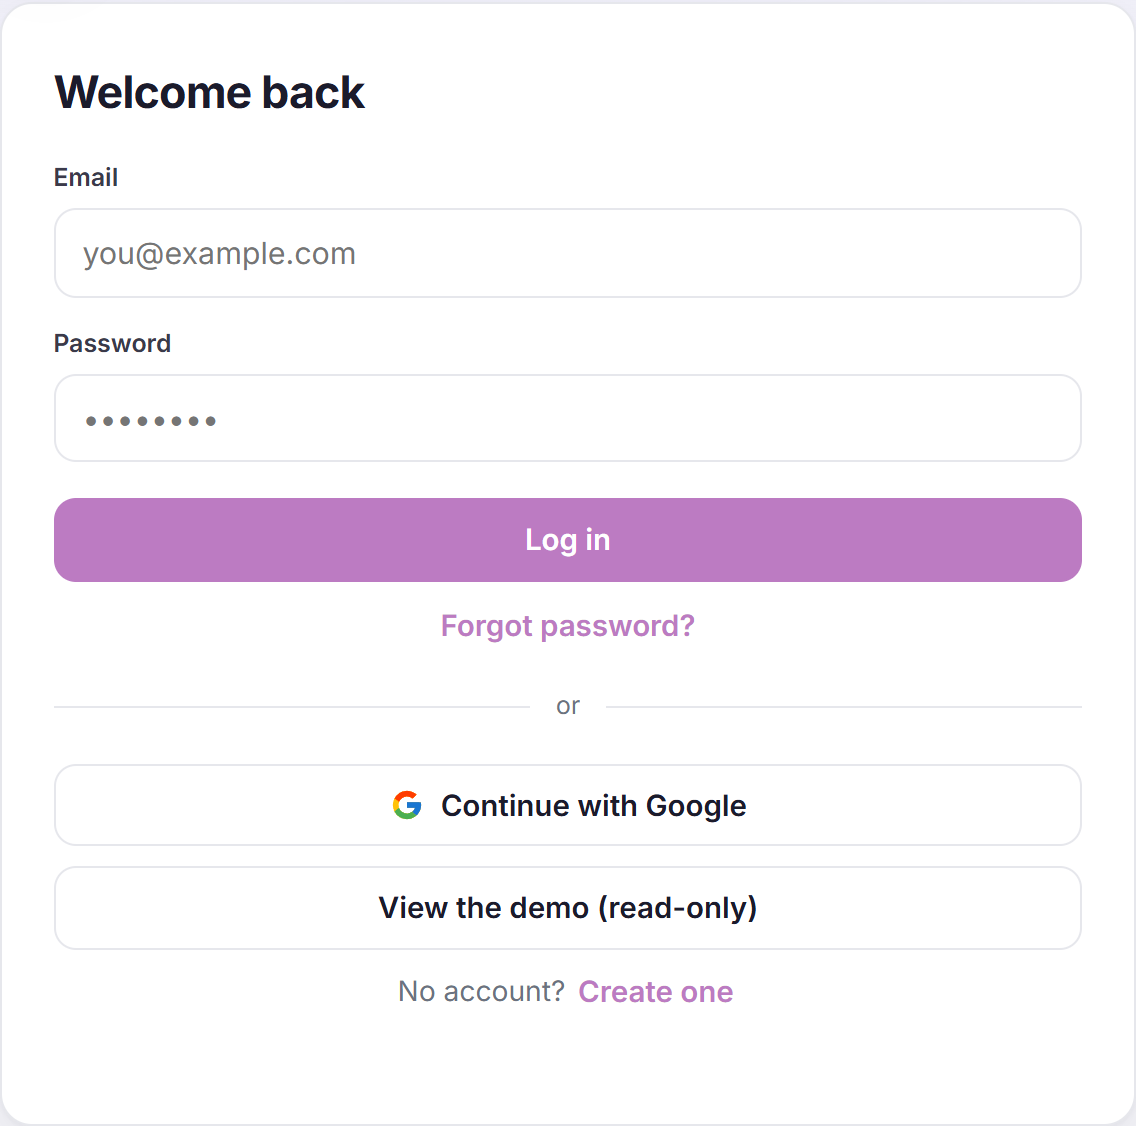
\includegraphics[width=0.5\textwidth]{ui-login.png}
  \caption{The sign-in front door: email/password, Google sign-in, the read-only demo, account
           creation, and password reset.}
  \label{fig:ui-login}
\end{figure}

\subsection{App navigation}

\Cref{fig:gui-flow} shows the journey through the screens. The front door leads to the dashboard
(by signing in, or read-only via the demo). From the dashboard a developer account can open the
console, and any owner can reach the account page or log out. The console hosts the training loop,
capture, label, train, then switch to production, after which detections appear back on the dashboard.

\begin{figure}[ht]\centering
  \resizebox{\textwidth}{!}{%
  \begin{tikzpicture}[node distance=11mm and 20mm, every node/.style={font=\footnotesize}]
    \node[mwterm] (land) {Sign-in front door};
    \node[mwnode, right=of land] (dash) {Dashboard\\\scriptsize live $\cdot$ health $\cdot$ history};
    \node[mwnode, above=10mm of dash] (acct) {Account\\\scriptsize devices $\cdot$ export $\cdot$ delete};
    \node[mwnode, right=of dash] (dev) {Dev console};
    \node[mwpill, below=12mm of dash, xshift=-6mm] (cap) {capture};
    \node[mwpill, right=10mm of cap] (lab) {label};
    \node[mwpill, right=10mm of lab] (tr) {train};
    \node[mwpill, right=10mm of tr] (run) {production};
    \draw[mwedge] (land) -- node[above,text=mwmut]{sign in / Google} (dash);
    \draw[mwedge] (dash) -- node[right,text=mwmut]{account} (acct);
    \draw[mwedge] (dash) -- node[above,text=mwmut]{dev account} (dev);
    \draw[mwedge] (dash.south west) to[bend right=12] node[below,text=mwmut,pos=0.4]{log out} (land.south east);
    \draw[mwedge] (dev) |- (run);
    \draw[mwedge] (cap) -- (lab);
    \draw[mwedge] (lab) -- (tr);
    \draw[mwedge] (tr) -- (run);
    \draw[mwedge] (run) |- (dash);
  \end{tikzpicture}}
  \caption{The user journey: front door to dashboard (or demo), the dashboard's branches to the
           account page and developer console, and the console's capture\,$\to$\,label\,$\to$\,train\,$\to$\,production
           loop that feeds detections back to the dashboard.}
  \label{fig:gui-flow}
\end{figure}

\subsection{The developer console}

The developer console is where training data is collected and models are trained
(\cref{sec:dashboard,sec:training-pipeline}). It is organised as collapsible cards, each with a
\texttt{?} help popover, described below in order.

\paragraph{Collar capture (\cref{fig:dev-collar}).} Live per-station status: which station and the
collar in range, the signal strength (RSSI) and whether the collar is within the capture threshold,
the station's power source, the collar's battery, how many collars are registered, and how long since
the station was last heard. The operator uses this to confirm a collar is close enough to record before
starting a capture.

\begin{figure}[ht]\centering
  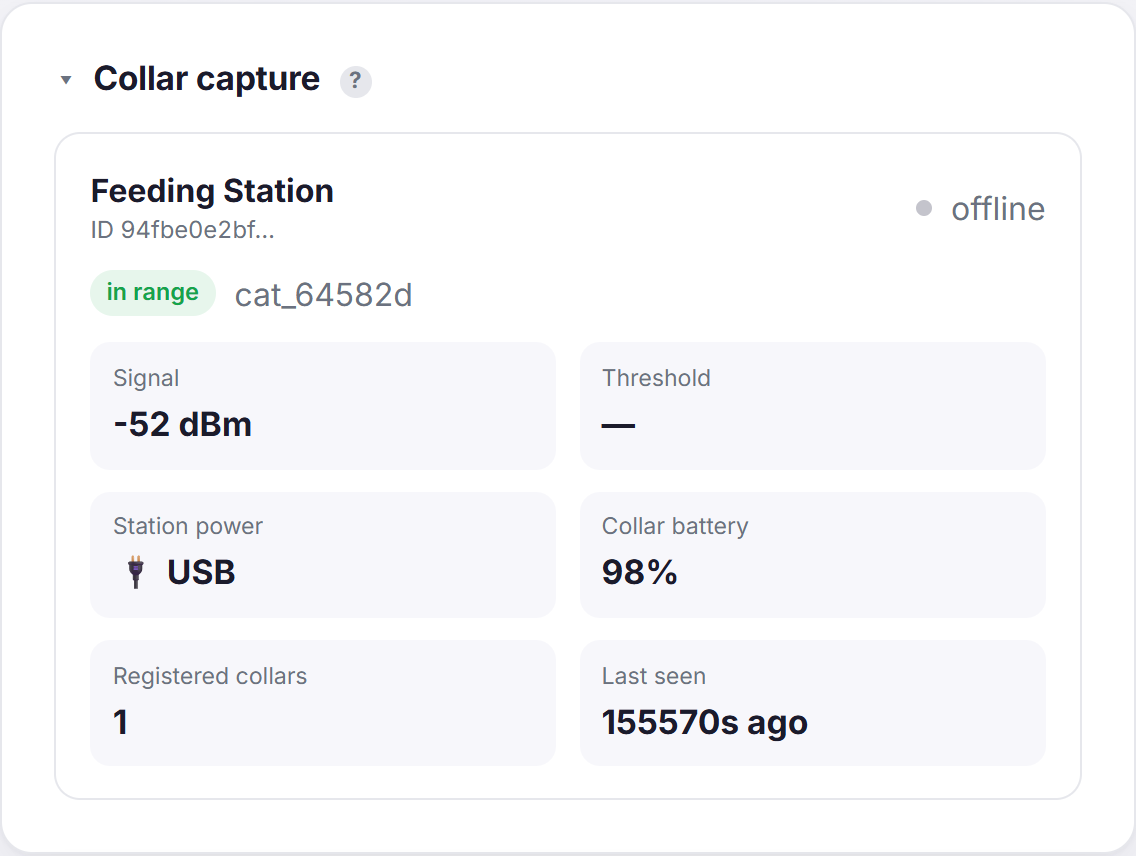
\includegraphics[width=0.72\textwidth]{ui-dev-collar.png}
  \caption{Collar capture: live station and collar status.}
  \label{fig:dev-collar}
\end{figure}

\paragraph{Mode (\cref{fig:dev-mode}).} A single switch between \textbf{Training} (the station records
and uploads clips) and \textbf{Production} (the station stops recording and only relays the collar's
on-device classification). This is the mode referenced throughout \cref{sec:architecture}.

\begin{figure}[ht]\centering
  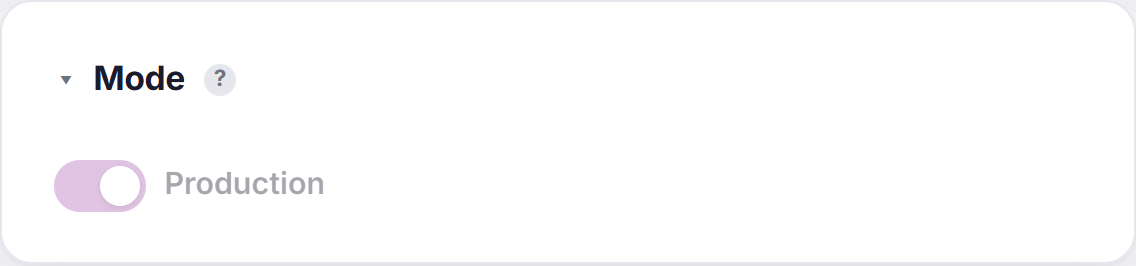
\includegraphics[width=0.6\textwidth]{ui-dev-mode.png}
  \caption{Mode: the Training\,/\,Production switch.}
  \label{fig:dev-mode}
\end{figure}

\paragraph{Actions to recognise (\cref{fig:dev-actions}).} The editable list of behaviours the system
should learn (here eat, drink, resting, moving). Adding or removing an action changes both the labels
offered when reviewing clips and the classes the cloud trainer learns, which makes the pipeline
label-agnostic (\cref{sec:training-pipeline}).

\begin{figure}[ht]\centering
  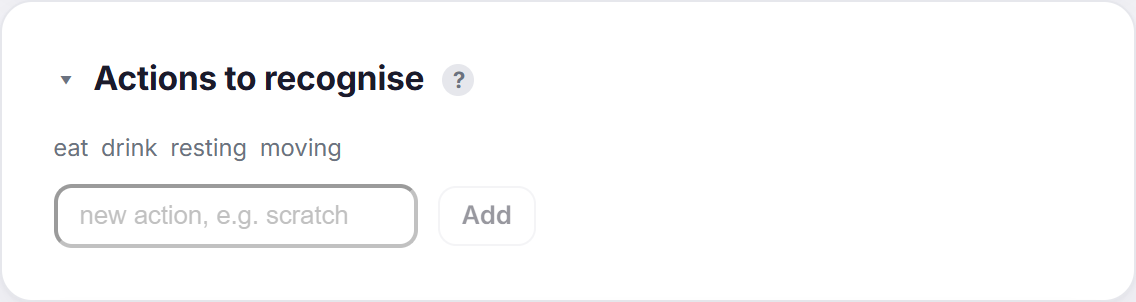
\includegraphics[width=0.66\textwidth]{ui-dev-actions.png}
  \caption{Actions to recognise: the owner-defined label set.}
  \label{fig:dev-actions}
\end{figure}

\paragraph{Record an action / live label (\cref{fig:dev-record}).} The fastest way to gather data:
pick a clip length, press the button for what the cat is doing \emph{now}, and the station records a
clip at any distance and auto-labels it, so there is no labelling afterwards. A \textbf{Full screen}
button gives a large, phone-style set of buttons for use at the bowl. A warning appears when the
station is offline (as shown), since clips cannot be captured without it.

\begin{figure}[ht]\centering
  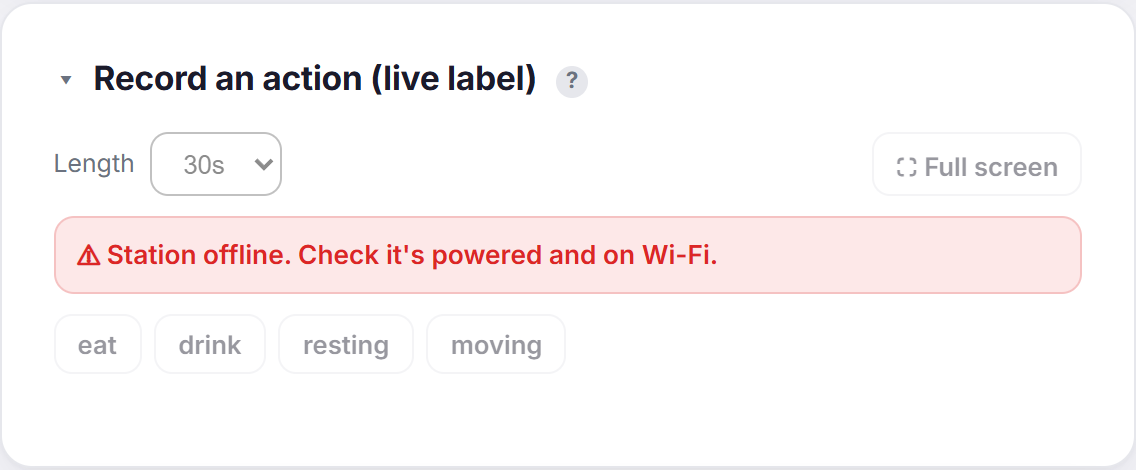
\includegraphics[width=0.78\textwidth]{ui-dev-record.png}
  \caption{Record an action (live label): length, category buttons, full-screen mode, and the
           station-offline warning.}
  \label{fig:dev-record}
\end{figure}

\paragraph{Bowl capture / label later (\cref{fig:dev-bowl}).} The alternative capture mode: with it on,
the station records back-to-back whenever a registered collar is within a configurable signal-strength
gate (with a dwell before it connects), and the clips are labelled afterwards in the clip review. It
suits behaviours that happen reliably at the bowl.

\begin{figure}[ht]\centering
  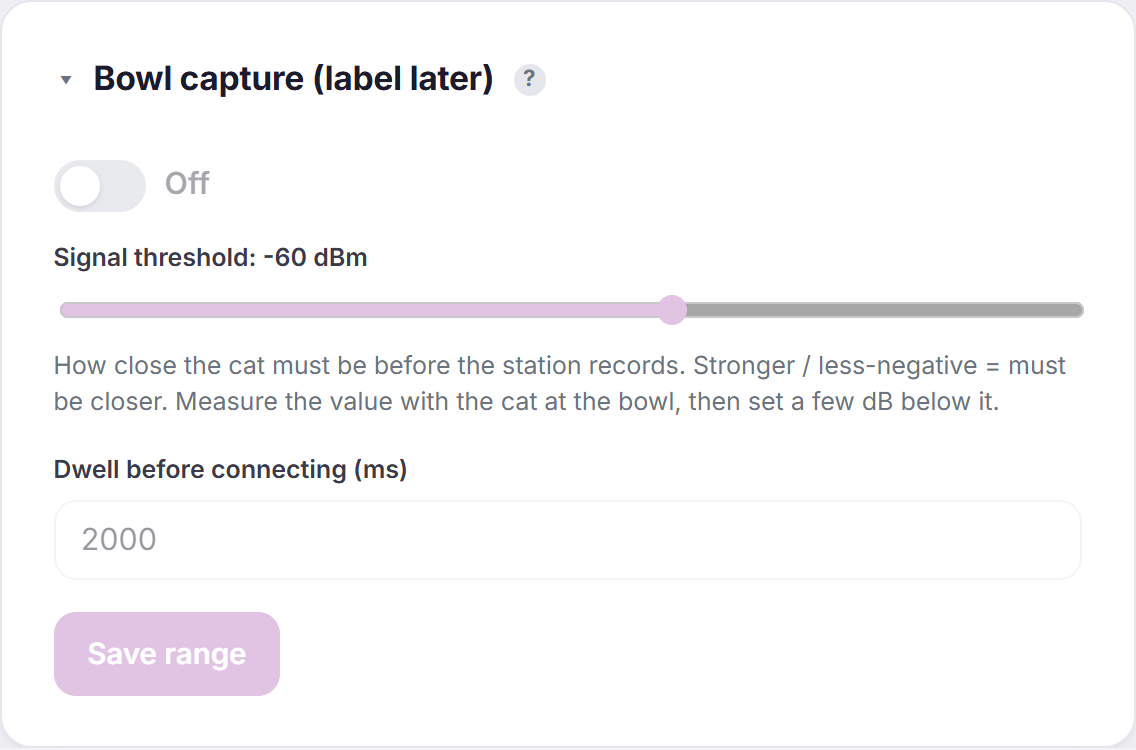
\includegraphics[width=0.72\textwidth]{ui-dev-bowl.png}
  \caption{Bowl capture: the range gate (signal threshold and dwell) for unattended recording.}
  \label{fig:dev-bowl}
\end{figure}

\paragraph{Recorded clips (\cref{fig:dev-clips}).} The dataset, and the richest card. Clips are grouped
by \textbf{day} and by \textbf{session} (a run of captures within the same few minutes), so a recording
run stays together. A per-label tally shows how many clips and sessions each action has, with a bar
toward a recommended minimum, so the operator sees at a glance which classes need more data.
\textbf{Analyse motion variety} scores how varied a label's samples are, a proxy for training quality
(too-similar samples generalise poorly). Each clip row carries a play control, a label dropdown, a
\textbf{Motion} badge when time-aligned IMU data is present, its time and length, and a delete control.
Clicking a clip expands it to a scrubber with the \emph{audio waveform and the motion (accelerometer
and gyroscope) traces drawn time-aligned beneath it}, plus draggable trim handles, so a sample can be
auditioned against its movement and tidied before training (\cref{fig:dev-expanded}). This expanded
view reads the clip's private audio and motion from Cloud Storage, so it is shown from a signed-in
account rather than the read-only demo.

\begin{figure}[ht]\centering
  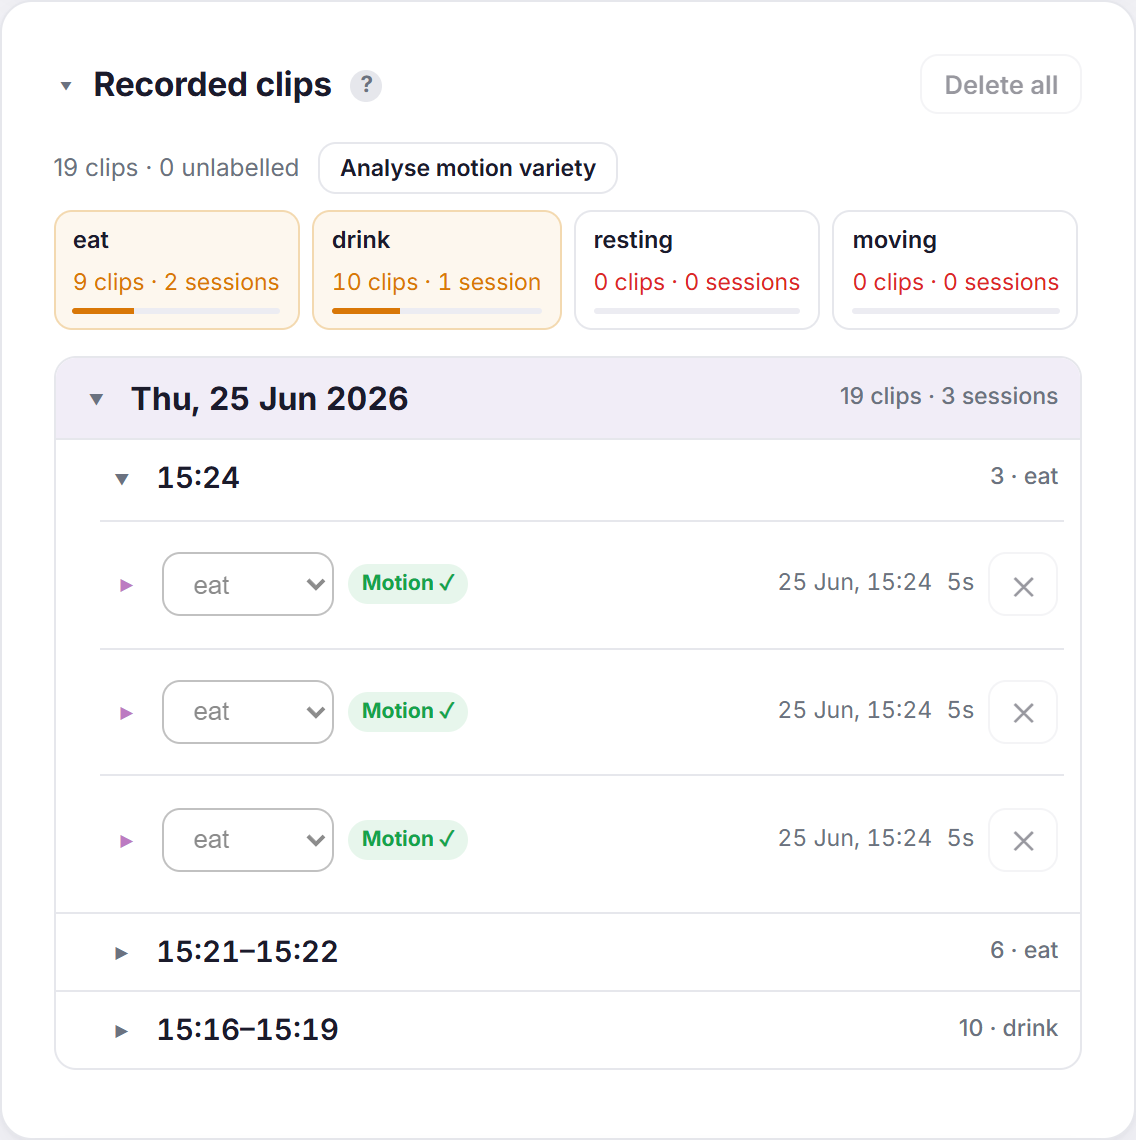
\includegraphics[width=0.74\textwidth]{ui-dev-clips.png}
  \caption{Recorded clips: per-label sample counts toward a minimum, the motion-variety quality check,
           and clips grouped by day and session, each with playback, a label, and a motion indicator.}
  \label{fig:dev-clips}
\end{figure}

\begin{figure}[ht]\centering
  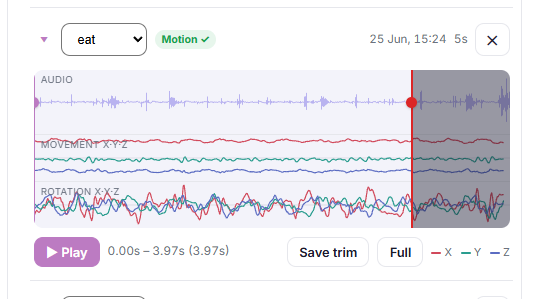
\includegraphics[width=0.78\textwidth]{ui-dev-label.png}
  \caption{A clip expanded for labelling: the audio waveform with the movement (accelerometer X/Y/Z)
           and rotation (gyroscope X/Y/Z) traces drawn time-aligned beneath it, plus draggable trim
           handles, a play control, and Save trim. The owner auditions the sound against the motion,
           confirms the label, and trims to the action before training.}
  \label{fig:dev-expanded}
\end{figure}

\paragraph{Train models (cloud) (\cref{fig:dev-train}).} \textbf{Retrain models} triggers the
\texttt{train} Cloud Function on the labelled clips (\cref{sec:training-pipeline}). The line below
reports live status, the current model version, and each stage's test accuracy and size (here an IMU
stage and an audio stage). When training finishes, the new version is delivered to the collar over the
air automatically (\cref{fig:training-flow}).

\begin{figure}[ht]\centering
  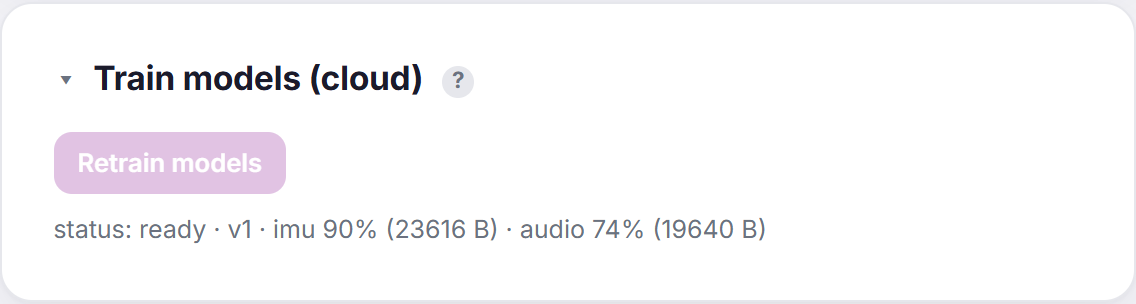
\includegraphics[width=0.66\textwidth]{ui-dev-train.png}
  \caption{Train models (cloud): the retrain trigger and the live training status (version and
           per-stage accuracy).}
  \label{fig:dev-train}
\end{figure}
